\documentclass[12pt]{article}
\usepackage{indentfirst}
\usepackage{amsmath}
\usepackage{multicol}
\setlength{\jot}{2ex}
\usepackage{mathrsfs}
\usepackage{graphicx}
\usepackage{wrapfig}
\usepackage{booktabs}
\usepackage[letterpaper, margin=1in]{geometry}
\usepackage{fancyhdr}
\usepackage{enumitem}
\usepackage[autostyle, english = american]{csquotes}
\MakeOuterQuote{"}
\renewcommand{\baselinestretch}{1.0}
\newcommand{\objects}[2]{%
  \leavevmode\vbox{\hbox{#1}\nointerlineskip\hbox{#2}}%
}
\title{Lab 2 \\ RLC Series Step Response}
\author{Qadis Chaudhry}
\date{October 25, 2021}
\begin{document}
\maketitle
    \section*{Introduction}
    \par The objective of this lab is to examine the response generated when connecting a source to a series configuration of an RLC network. With this configuration, we have two energy storing elements, the inductor and the capacitor, which attributes an oscillatory evolution to the current or voltage in the circuit. The dampening of this oscillation is controlled by the introduction of the resistor. This acts to reduce the oscillation as it is a passive element; the higher the resistance, the more damped the oscillation.
    \par By examining the equations which dictate the behavior of such a circuit, we can see how the values of the constants related to each of the elements determine the evolution of the setup. The natural and damped frequencies arise as combinations of these three values and it will be seen that the increase in the value of the resistance will directly translate to changes within the oscillation.
    \section*{Prelab Exercises}
    \begin{itemize}
        \item[3.1]
    \end{itemize}
    \par Since the natural frequency $ \omega_0 $ is represented by the values of $ L $ and C, and the values of L and $ \omega_0 $ are known, we can determine an expression for $ C $ and plug in the known values to determine its value.
    \begin{align*}
        \omega_0 &= \frac{1}{\sqrt{LC}} \\
        C &= \frac{1}{\omega_0^2 L}
    \end{align*}
    Plugging in the values for $ L $ and $ \omega_0 $ we get a value for $ C $,
    \[
        C = \frac{1}{(10^{4} \pi)^2(100 \times 10^{-3})} = \boxed{10.13\ \text{nF}}
    \]
    Now, to find the value of $ R $ based on the given damping coefficients we can use the equation,
    \[
        \zeta = \frac{R}{2} \sqrt{\frac{C}{L}}
    \]
    where the only unknown is the variable $ R $ which we can solve for.
    \[
        R = 2 \zeta \sqrt{\frac{L}{C}}
    \]
    Using this equation along with each of the different values of $ \zeta $, we can get all the different required values of $ R $.
    \begin{table}[h]
        \centering
        \begin{tabular}{ccc}
            \toprule
            $ \zeta $ & $ 2 \zeta \sqrt{\frac{L}{C}} $ & $ R $ \\
            \midrule
            0.1 & $ 2 (0.1) \sqrt{\frac{100 \times 10^{-3}}{10.13 \times 10^{-9}}} $ & 628.32 $ \Omega $ \\
            0.2 & $ 2 (0.2) \sqrt{\frac{100 \times 10^{-3}}{10.13 \times 10^{-9}}} $ & 1256.64 $ \Omega $ \\
            0.4 & $ 2 (0.4) \sqrt{\frac{100 \times 10^{-3}}{10.13 \times 10^{-9}}} $ & 2513.27 $ \Omega $ \\
            0.6 & $ 2 (0.6) \sqrt{\frac{100 \times 10^{-3}}{10.13 \times 10^{-9}}} $ & 3769.91 $ \Omega $ \\
            0.8 & $ 2 (0.8) \sqrt{\frac{100 \times 10^{-3}}{10.13 \times 10^{-9}}} $ & 5026.55 $ \Omega $ \\
            1.0 & $ 2 (1.0) \sqrt{\frac{100 \times 10^{-3}}{10.13 \times 10^{-9}}} $ & 6283.19 $ \Omega $ \\
            \bottomrule
        \end{tabular}
    \end{table}
    \begin{itemize}
        \item[3.2]
    \end{itemize}
    \par The equation we will use is defined as,
    \[
        v_{c} (k \pi / \omega_{d}) = 2 - 2(-1)^{k} e^{-k \pi \zeta / \sqrt{1- \zeta^2}}
    \]
    where the values of $ k $ will be 1, 2, and 3 for the calculations of the minima and the two maxima.
    \begin{table}[h]
        \centering
        \begin{tabular}{cccc}
            \toprule
            \multicolumn{4}{c}{Theoretical Values} \\
            \midrule
            $ \zeta $ & $ k = $ 1 & $ k = $ 2 & $ k = $ 3 \\
            \midrule
            0.1 & 3.4685 & 0.9364 & 2.7756 \\
            0.2 & 3.0532 & 1.4453 & 2.2921 \\
            0.4 & 2.5077 & 1.8711 & 2.0327 \\
            0.6 & 2.1896 & 1.9820 & 2.0017 \\
            0.8 & 2.0303 & 1.9995 & 2.0000 \\
            1.0 & undefined & undefined & undefined \\
            \bottomrule
        \end{tabular}
    \end{table}
    \\
    These are the theoretical values for the minima and maxima of the function that describes the voltage of the RLC circuit. The values of this table will later be compared with the measurements from the actual configuration.
    \section*{Experiments and Results}
    \begin{table}[h]
        \centering
        \begin{tabular}{cccc}
            \toprule
            \multicolumn{4}{c}{Measured Values} \\
            \midrule
            $ \zeta $ & Maximum 1 & Minimum & Maximum 2 \\
            \midrule
            0.1 & 3.16 & 0.94595 & 2.51 \\
            0.2 & 2.80 & 1.87 & 2.07 \\
            0.4 & 2.24 & 1.94 & 2.01 \\
            0.6 & 2.16 & 1.95 & 2.00 \\
            0.8 & 2.02 & 1.97 & 2.00 \\
            1.0 & 2.00 & 2.00 & 2.00 \\
            \bottomrule
        \end{tabular}
    \end{table}
    \begin{center}
        \objects
            {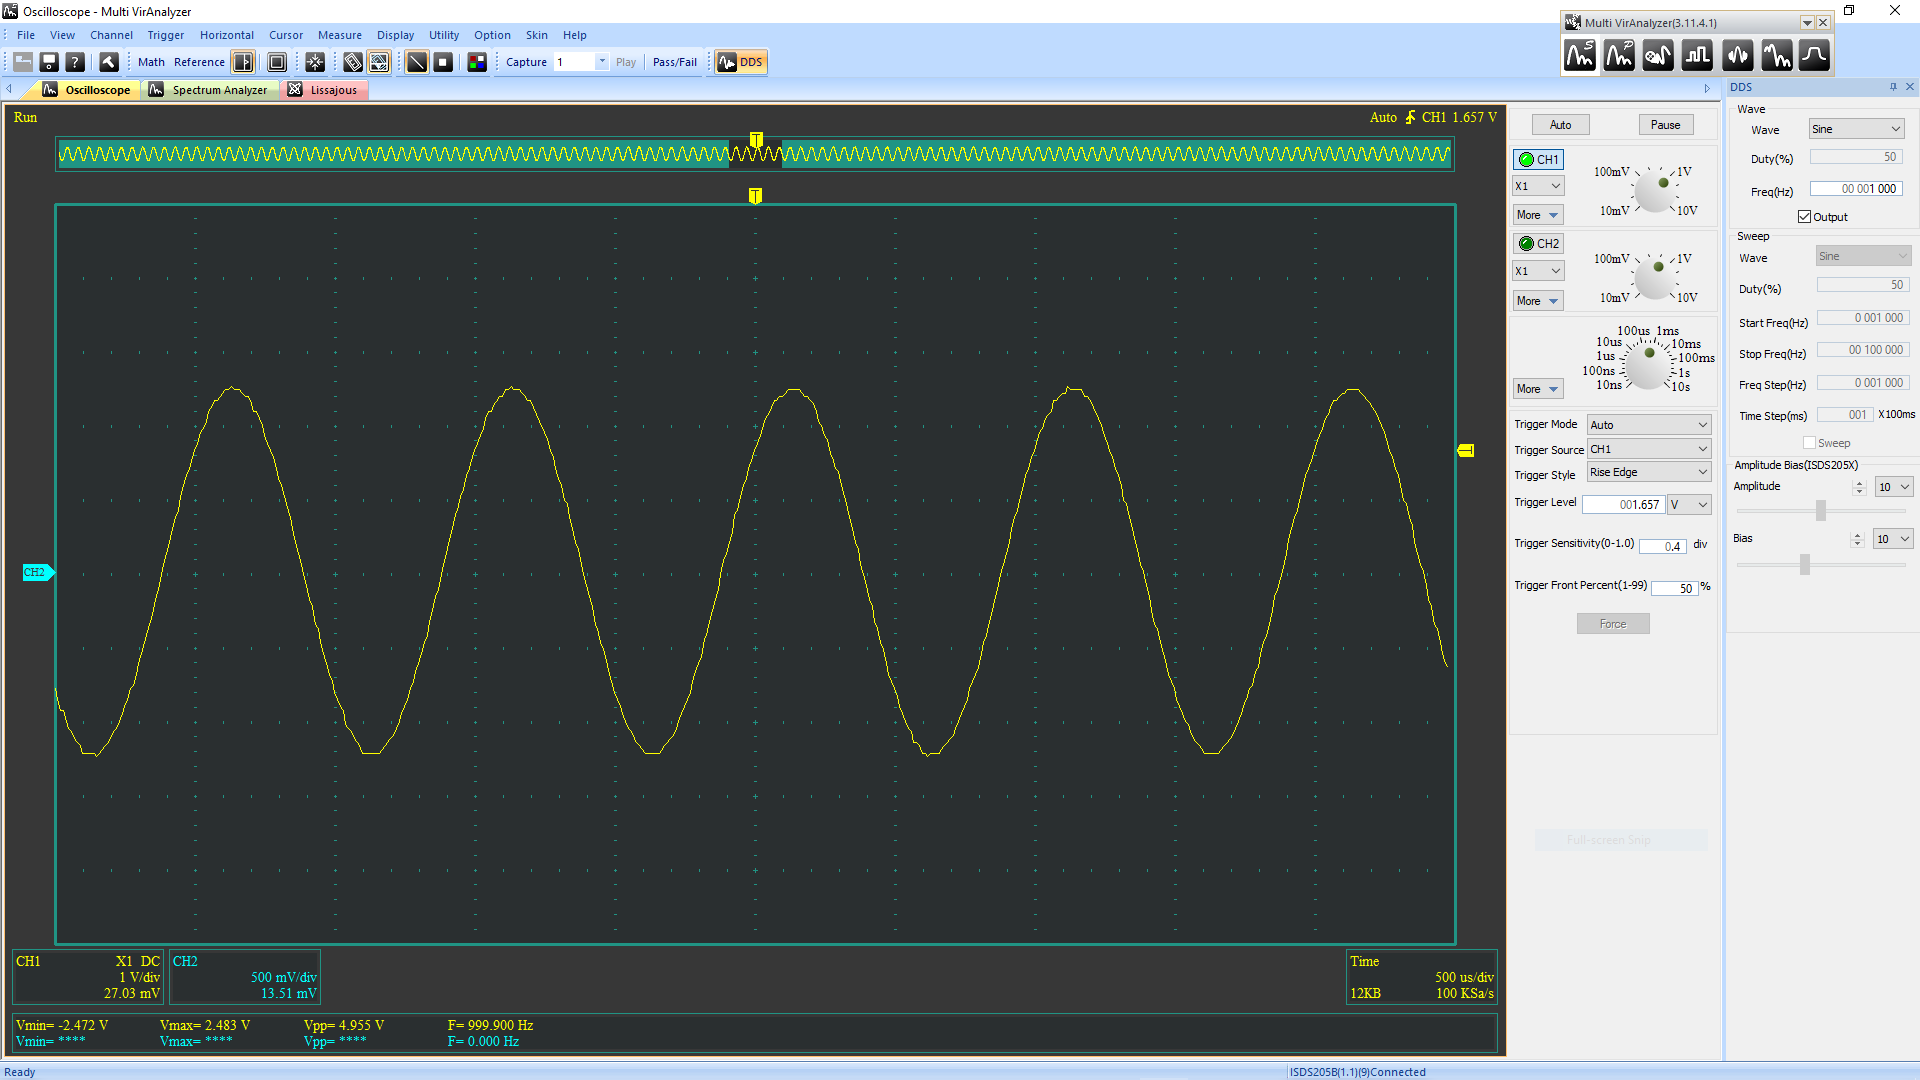
\includegraphics[width=0.7\textwidth]{4.1a.png}}
            {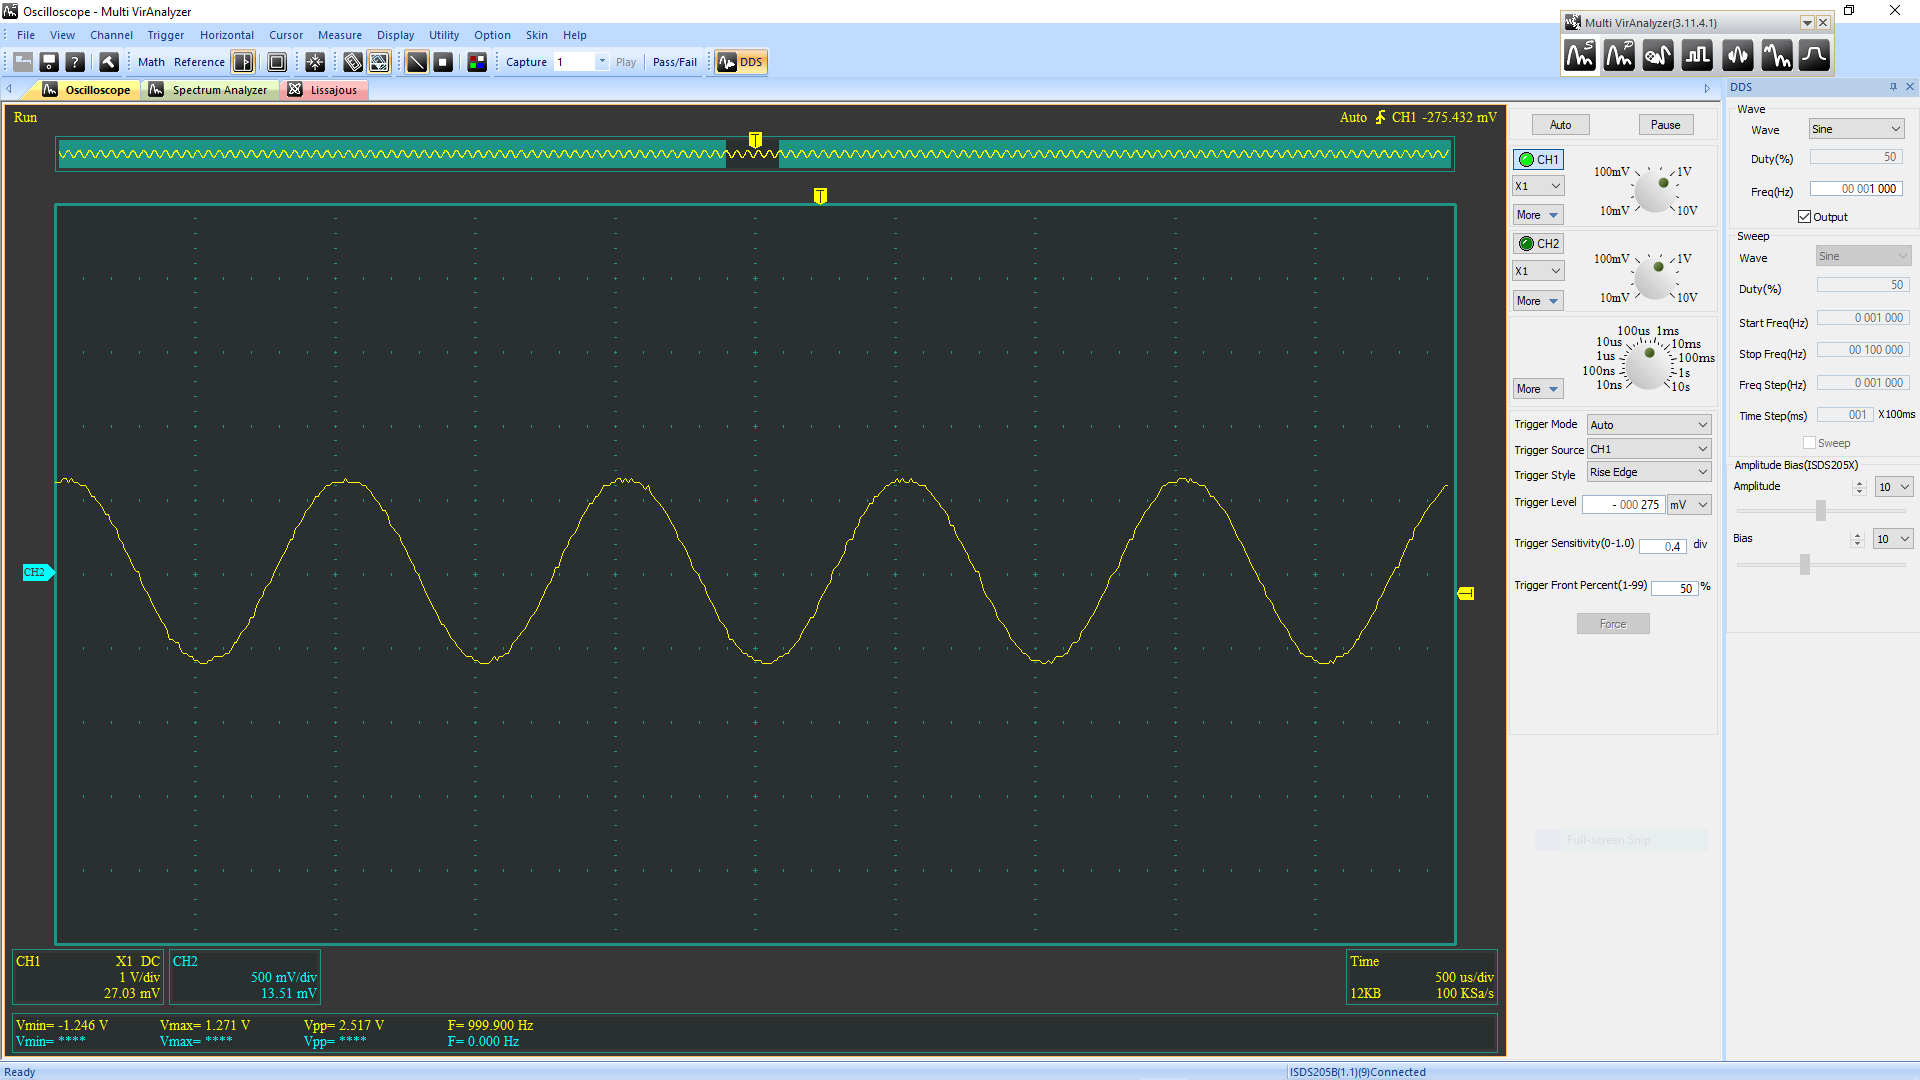
\includegraphics[width=0.7\textwidth]{4.1b.png}}
    \end{center}
    \begin{center}
        Figures for part 4.1. Top shows the sign wave with 5 V peak to peak, and the bottom shows the peak to peak of 2.5 V. From this, the value of the variable resistor is measured to find the value of the internal resistance of the function generator. This value was found to be 198 $ \Omega $.
    \end{center}
    \begin{figure}[h]
        \centering
        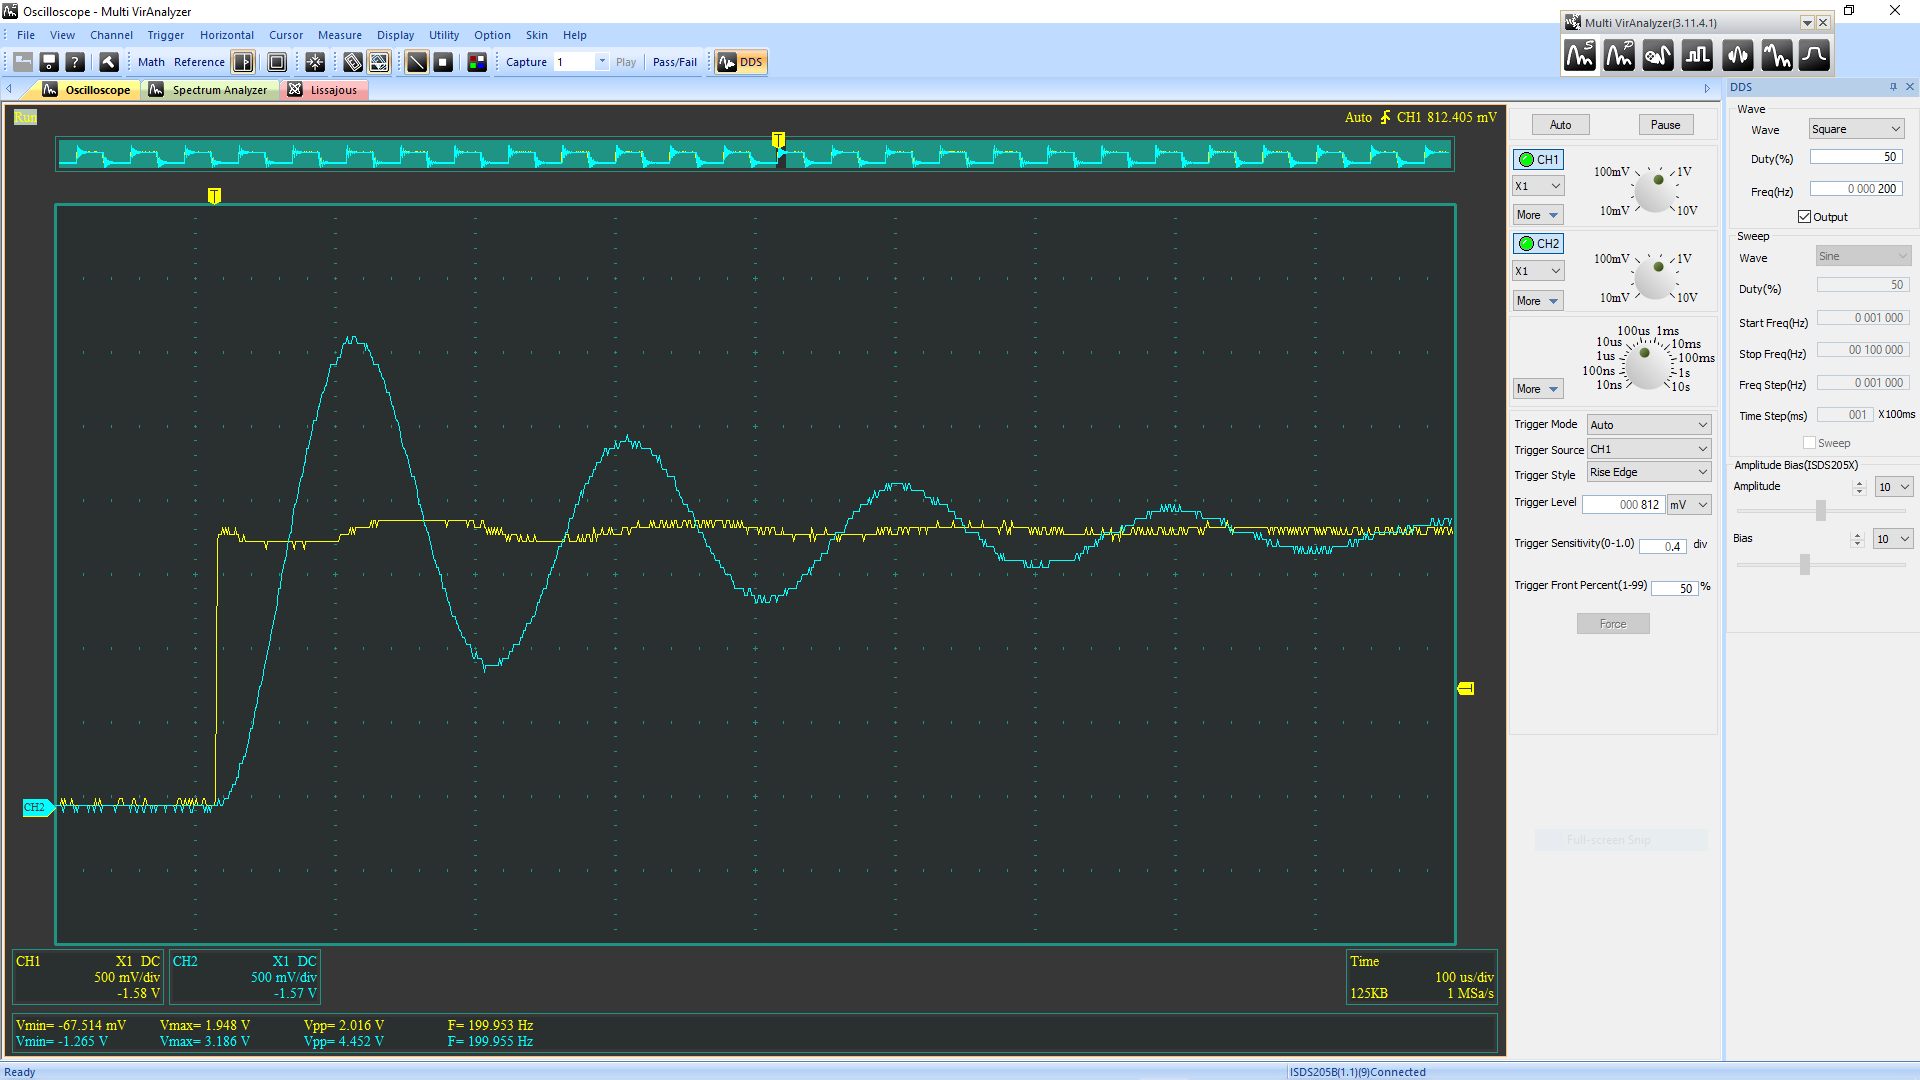
\includegraphics[width=\textwidth]{4.3.png}
        \caption{Step response generated in experiment 4.3}
    \end{figure}
    \par This is the step response of the RLC circuit. The oscillation can be seen to be damped and this is due to the internal resistances of the function generator as well as the inductor, along with the value of the variable resistor. Here the value of $ \zeta $ is 0.1, and the value of the variable resistor is set so the resistances of the inductor and the function generator are taken into account. The theoretical resistance for when $ \zeta = 0.1 $, is 628.32. From this we subtract the determined value of the function generator resistance, 198 $ \Omega $, and the resistance of the inductor, 220 $ \Omega $. This gives a value of the variable resistor, 210.32 $ \Omega $. With this setup we can alter the value of $ \zeta $ and examine the changes in the response of the circuit.
    \newpage
    \begin{center}
        \objects
            {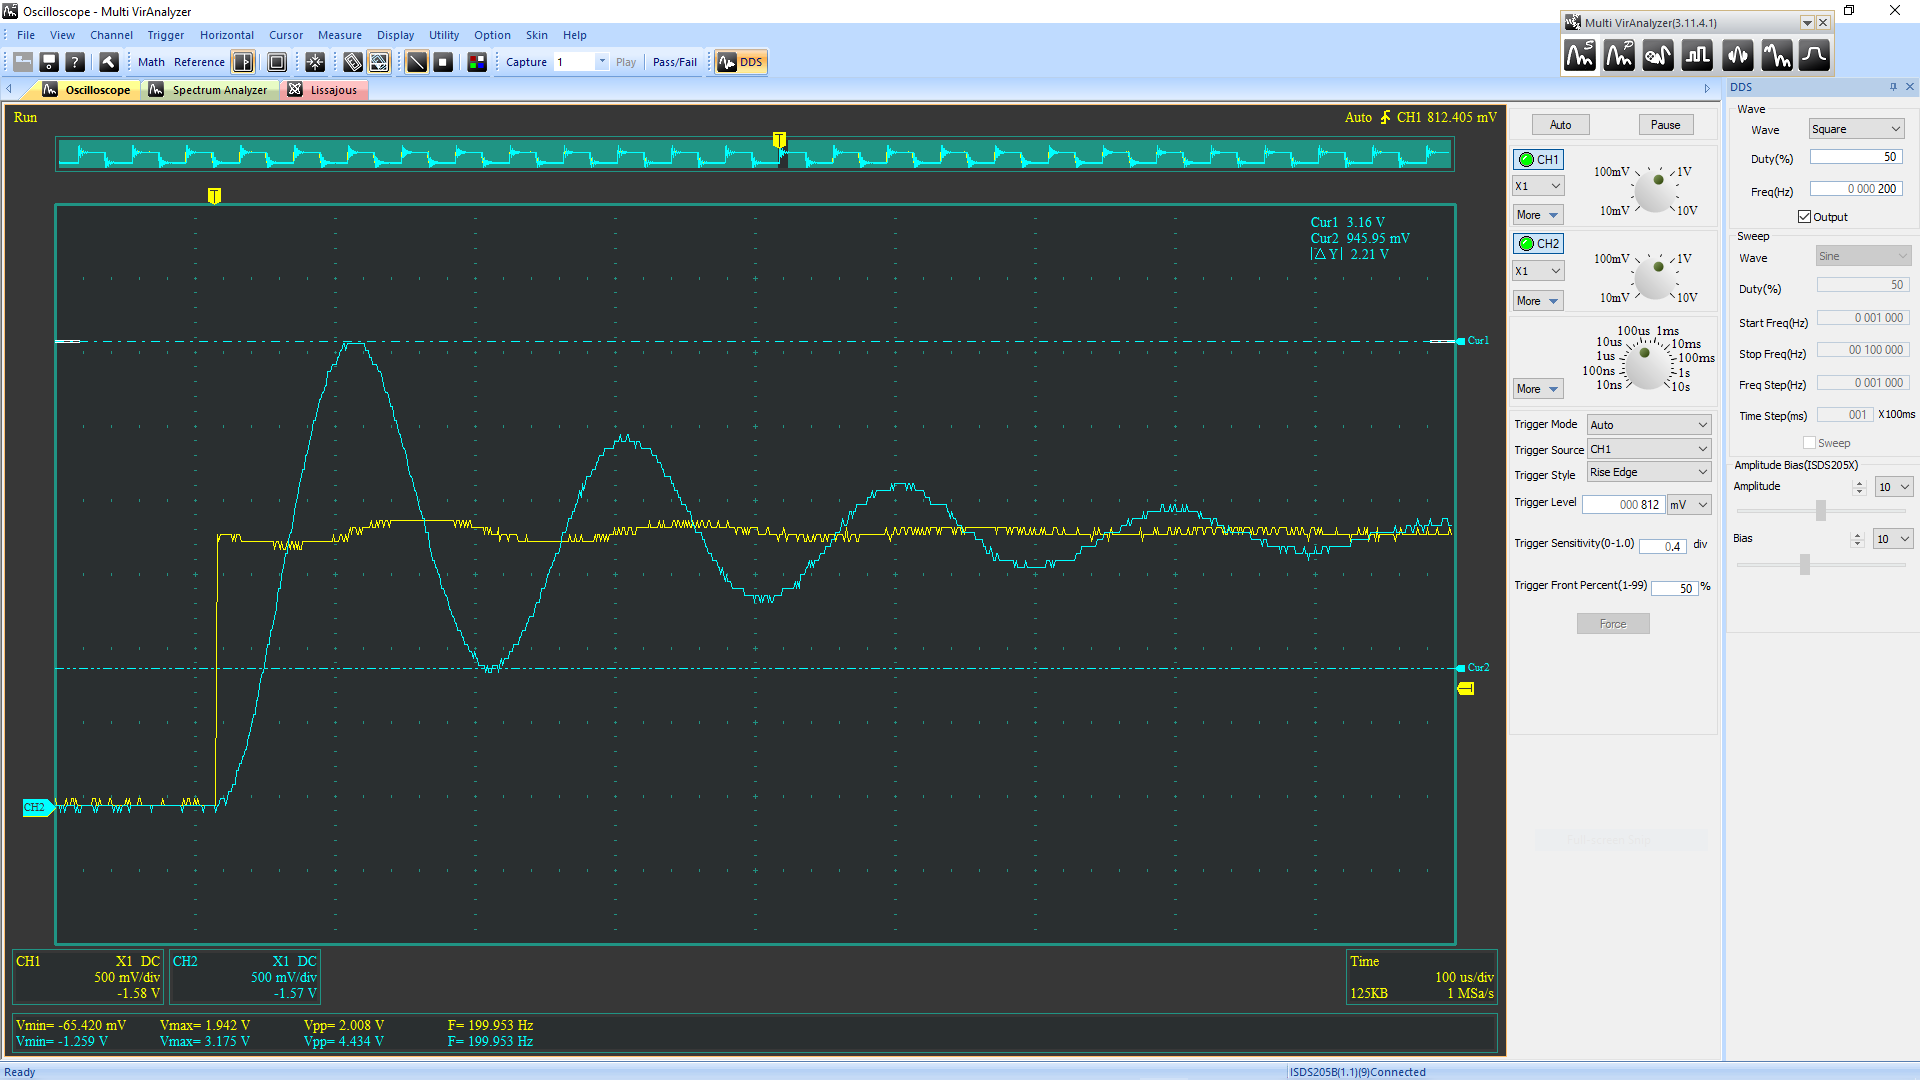
\includegraphics[width=\textwidth]{4.4 (0.1) 1.png}}
            {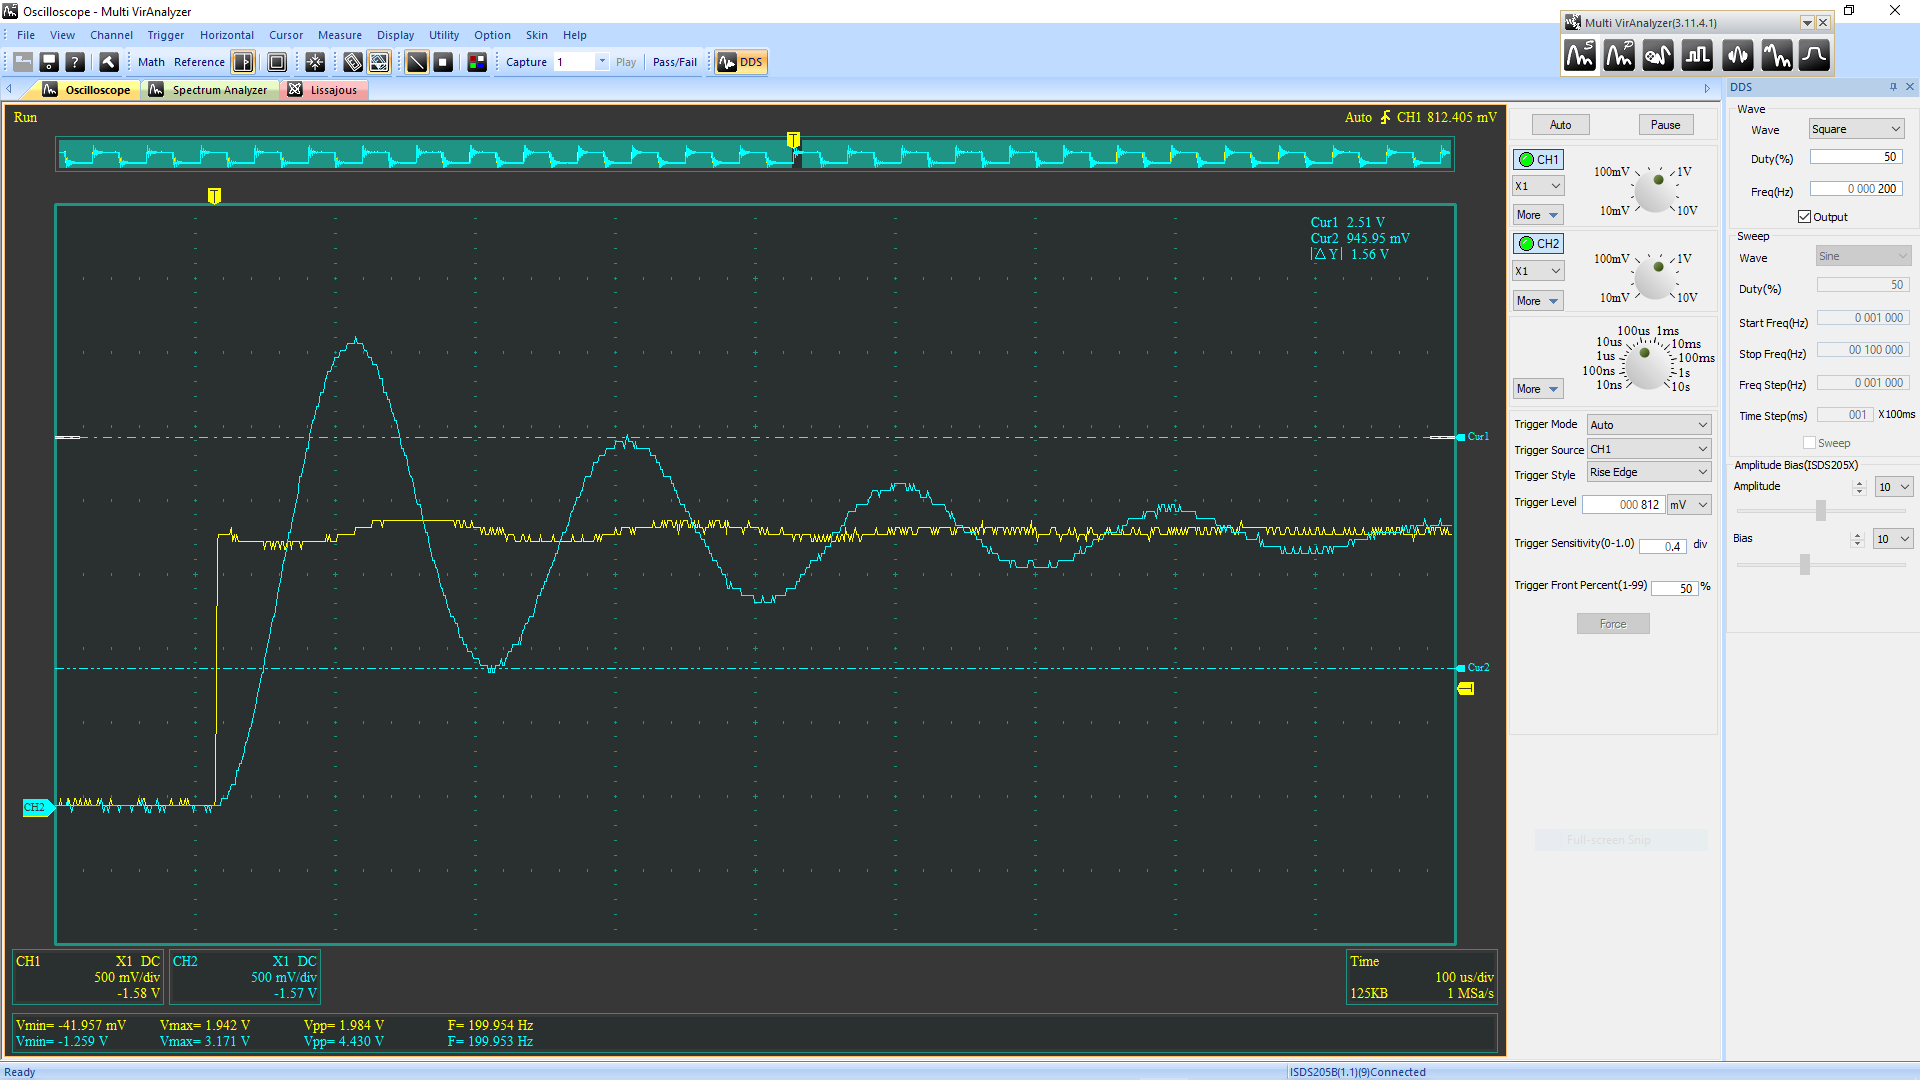
\includegraphics[width=\textwidth]{4.4 (0.1) 2.png}}
    \end{center}
    \begin{center}
        Figures 2 and 3: Step response of RLC when $ \zeta = 0.1 $, $ R = 210.32 \Omega $
    \end{center}
    \newpage
    \begin{center}
        \objects
            {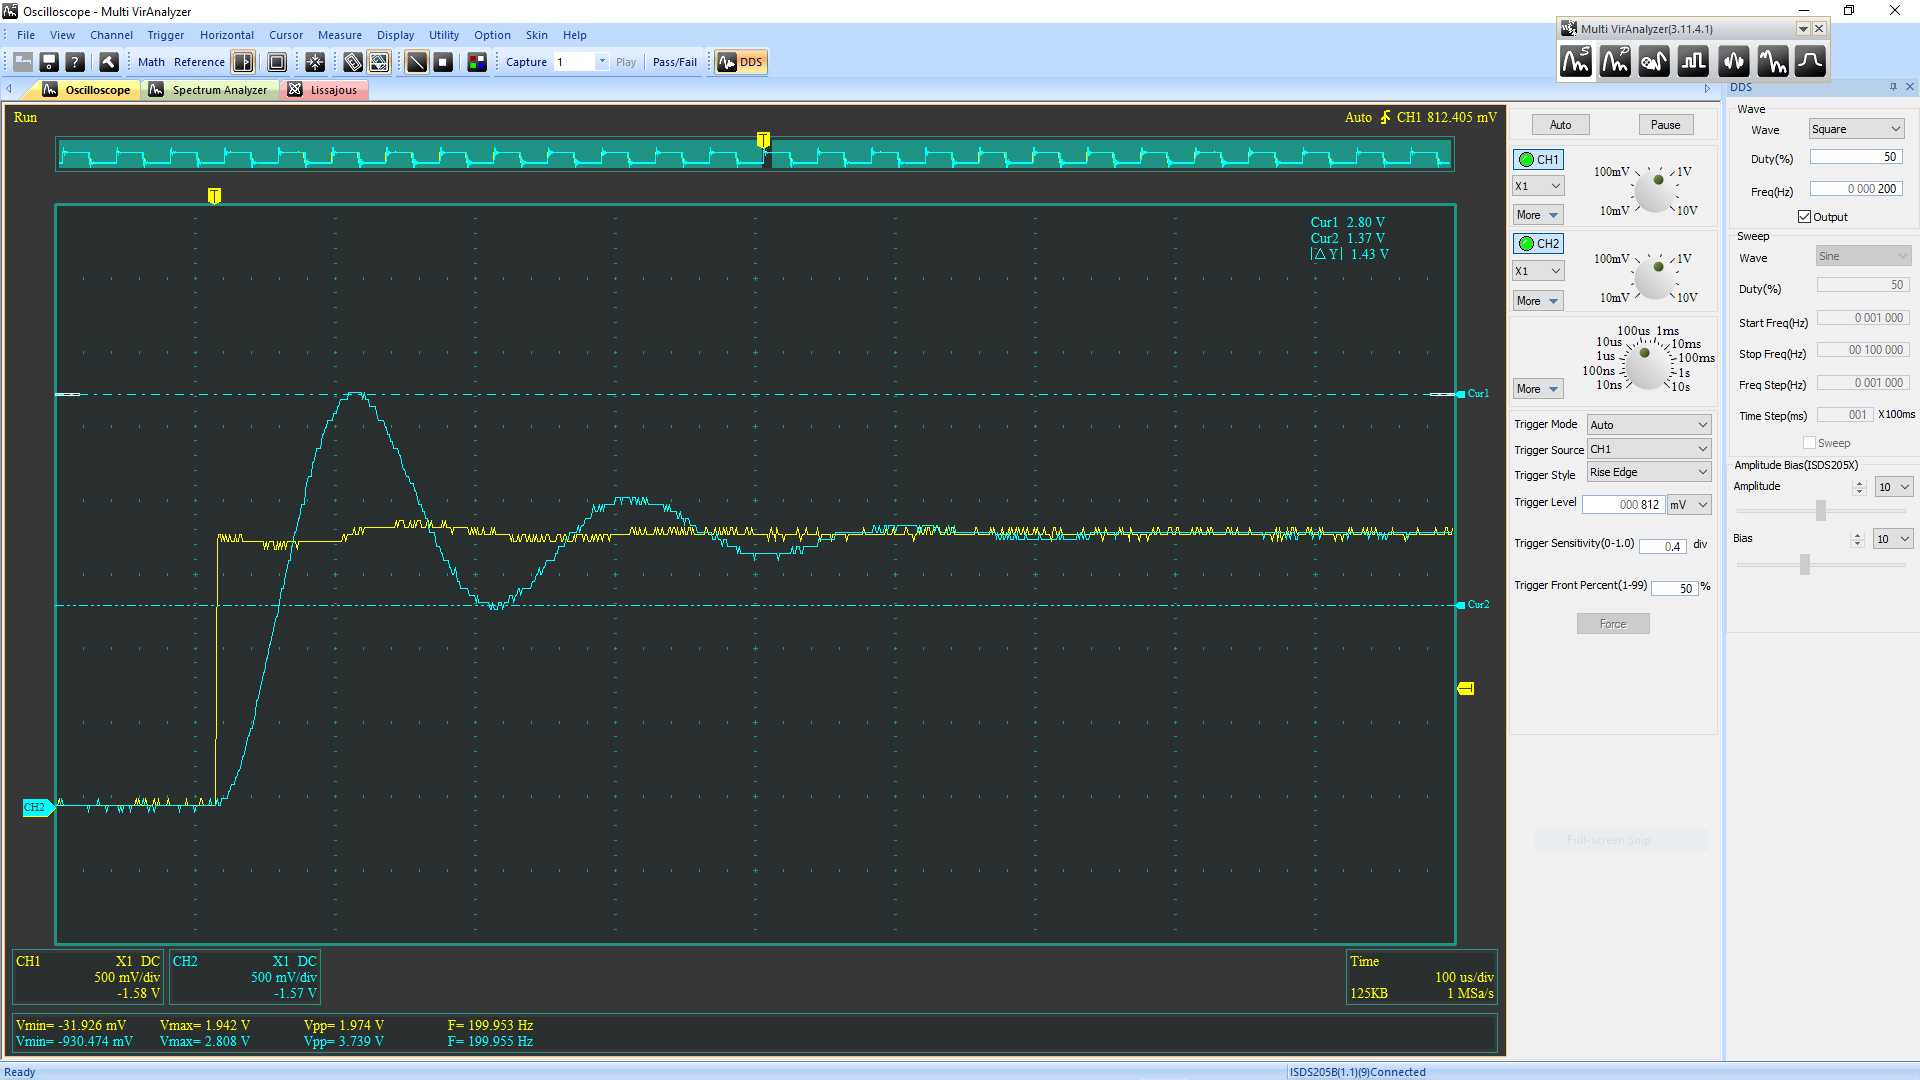
\includegraphics[width=\textwidth]{4.4 (0.2) 1.png}}
            {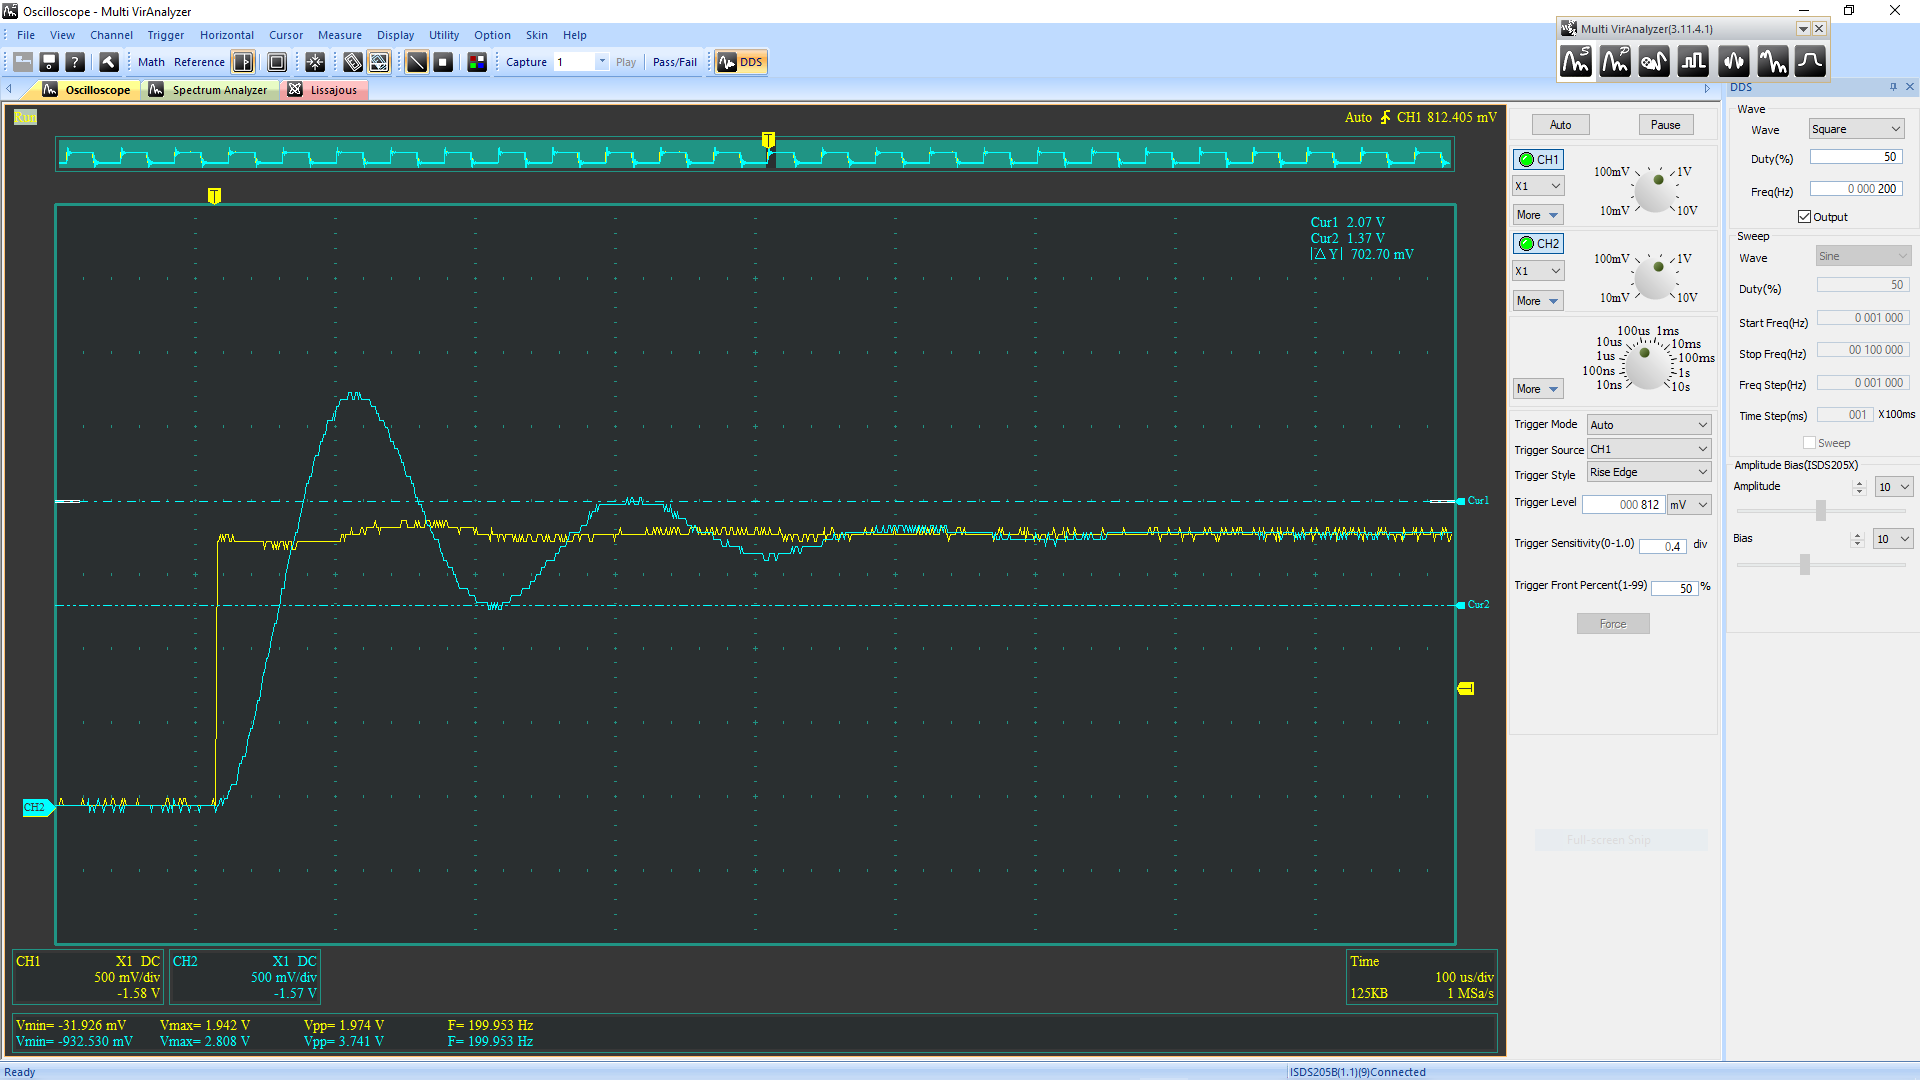
\includegraphics[width=\textwidth]{4.4 (0.2) 2.png}}
    \end{center}
    \begin{center}
        Figures 4 and 5: Step response when $ \zeta = 0.2 $, $ R = 838.64 \Omega $
    \end{center}
    \newpage
    \begin{center}
        \objects
            {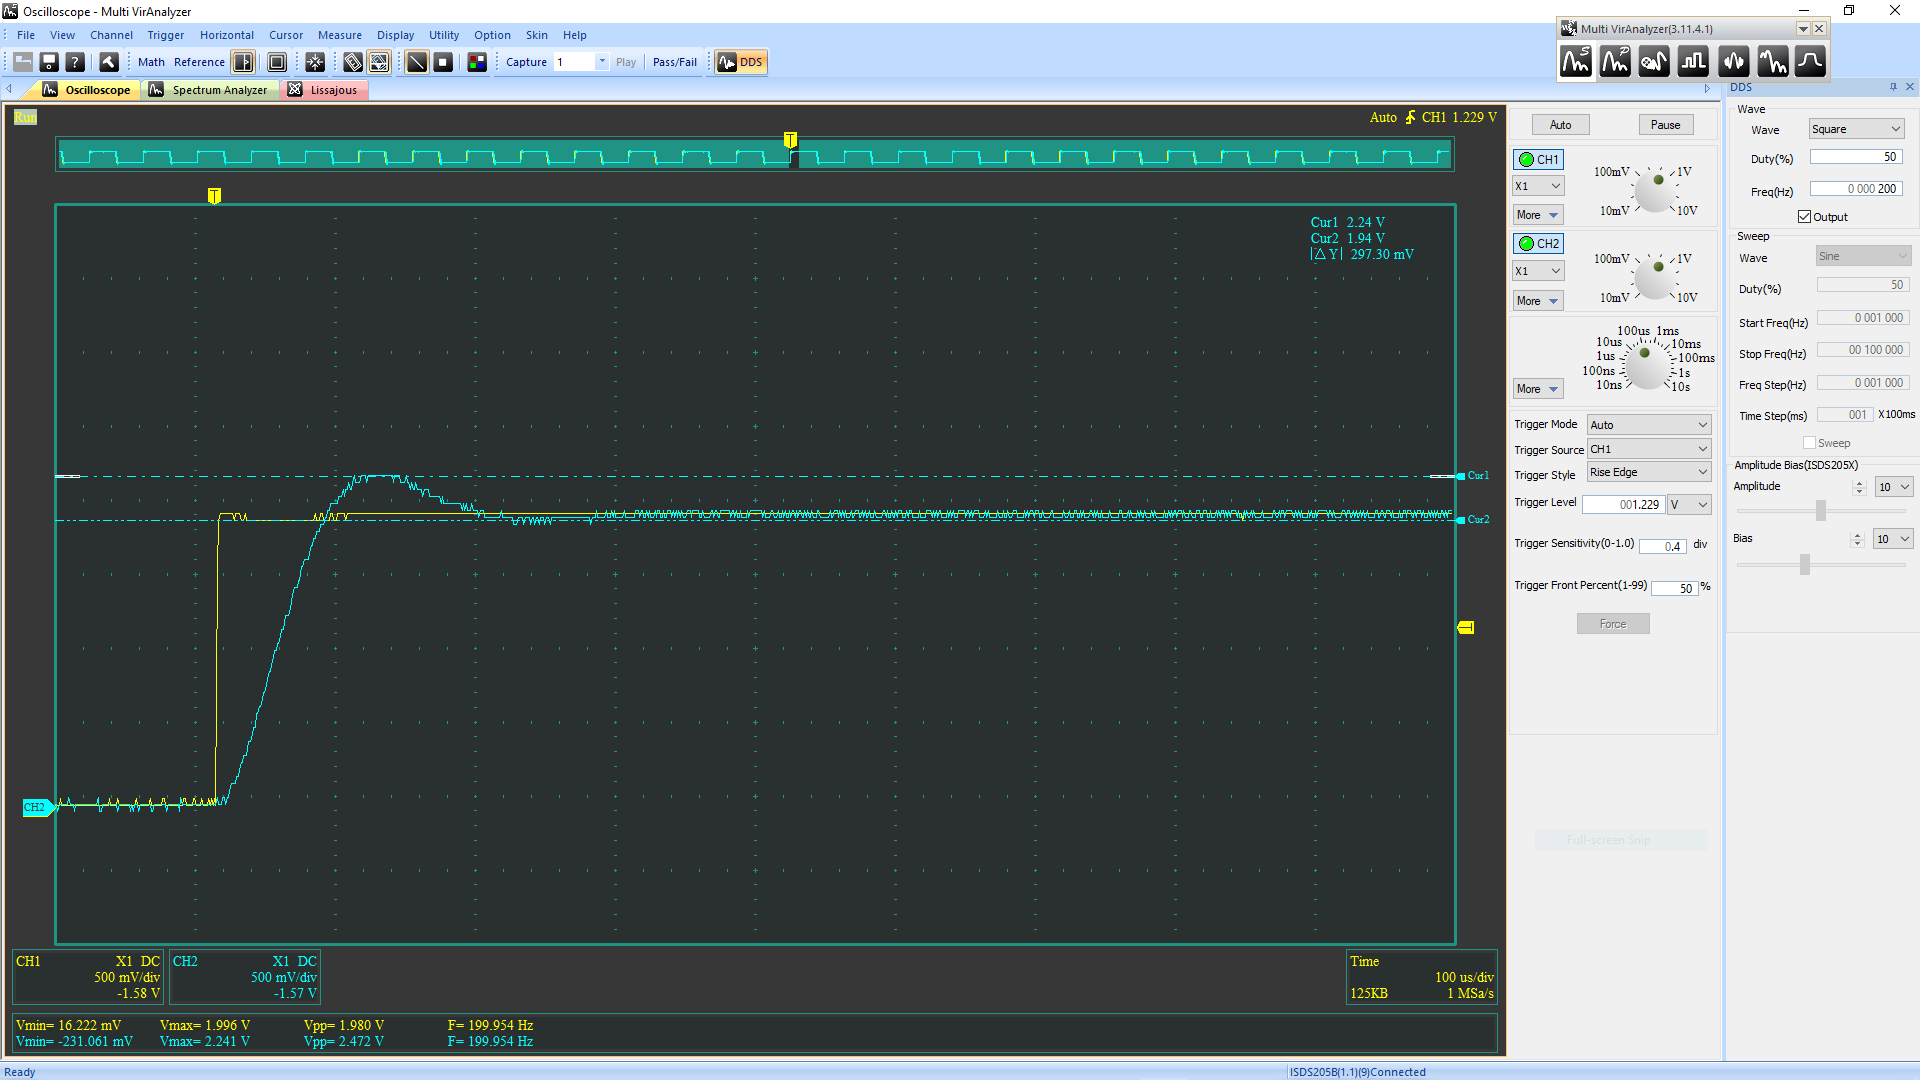
\includegraphics[width=\textwidth]{4.4 (0.4) 1.png}}
            {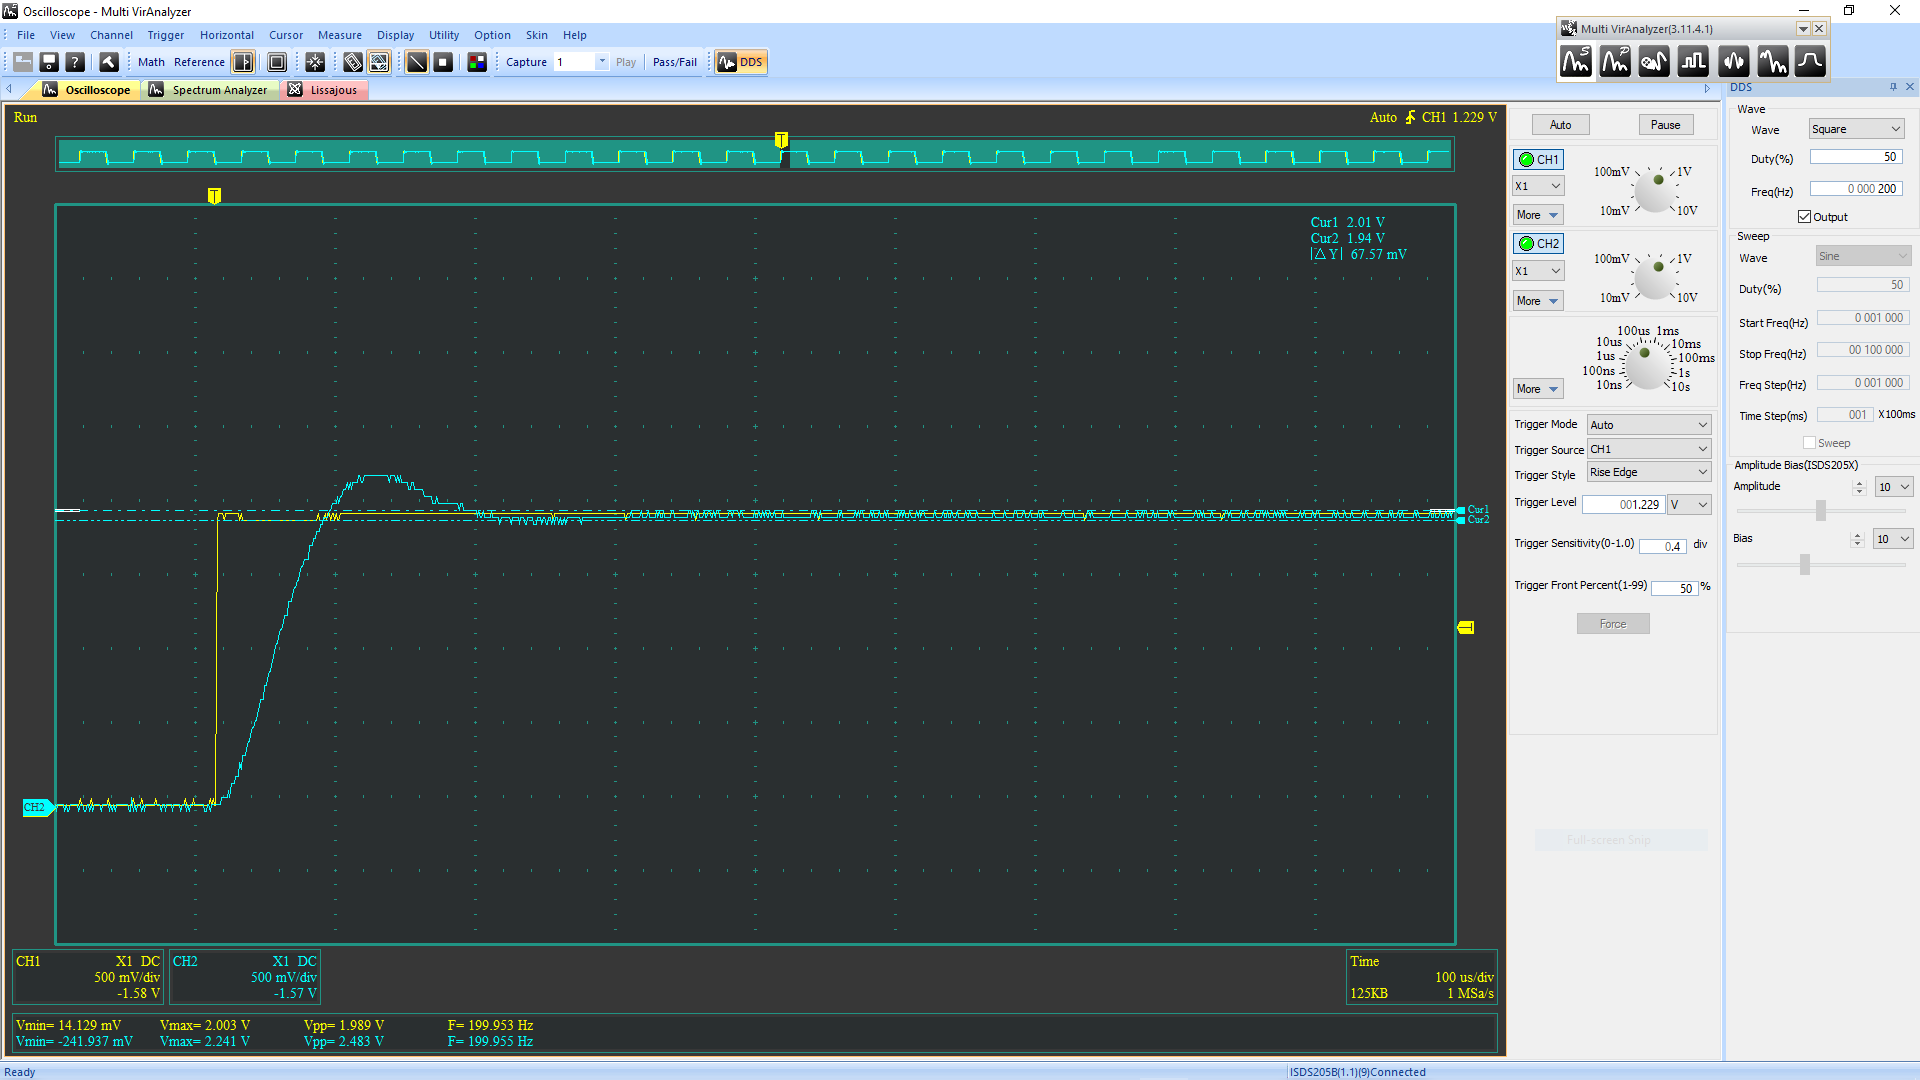
\includegraphics[width=\textwidth]{4.4 (0.4) 2.png}}
    \end{center}
    \begin{center}
        Figures 6 and 7: Step response when $ \zeta = 0.4 $, $ R = 2095.27 \Omega $
    \end{center}
    \newpage
    \begin{center}
        \objects
            {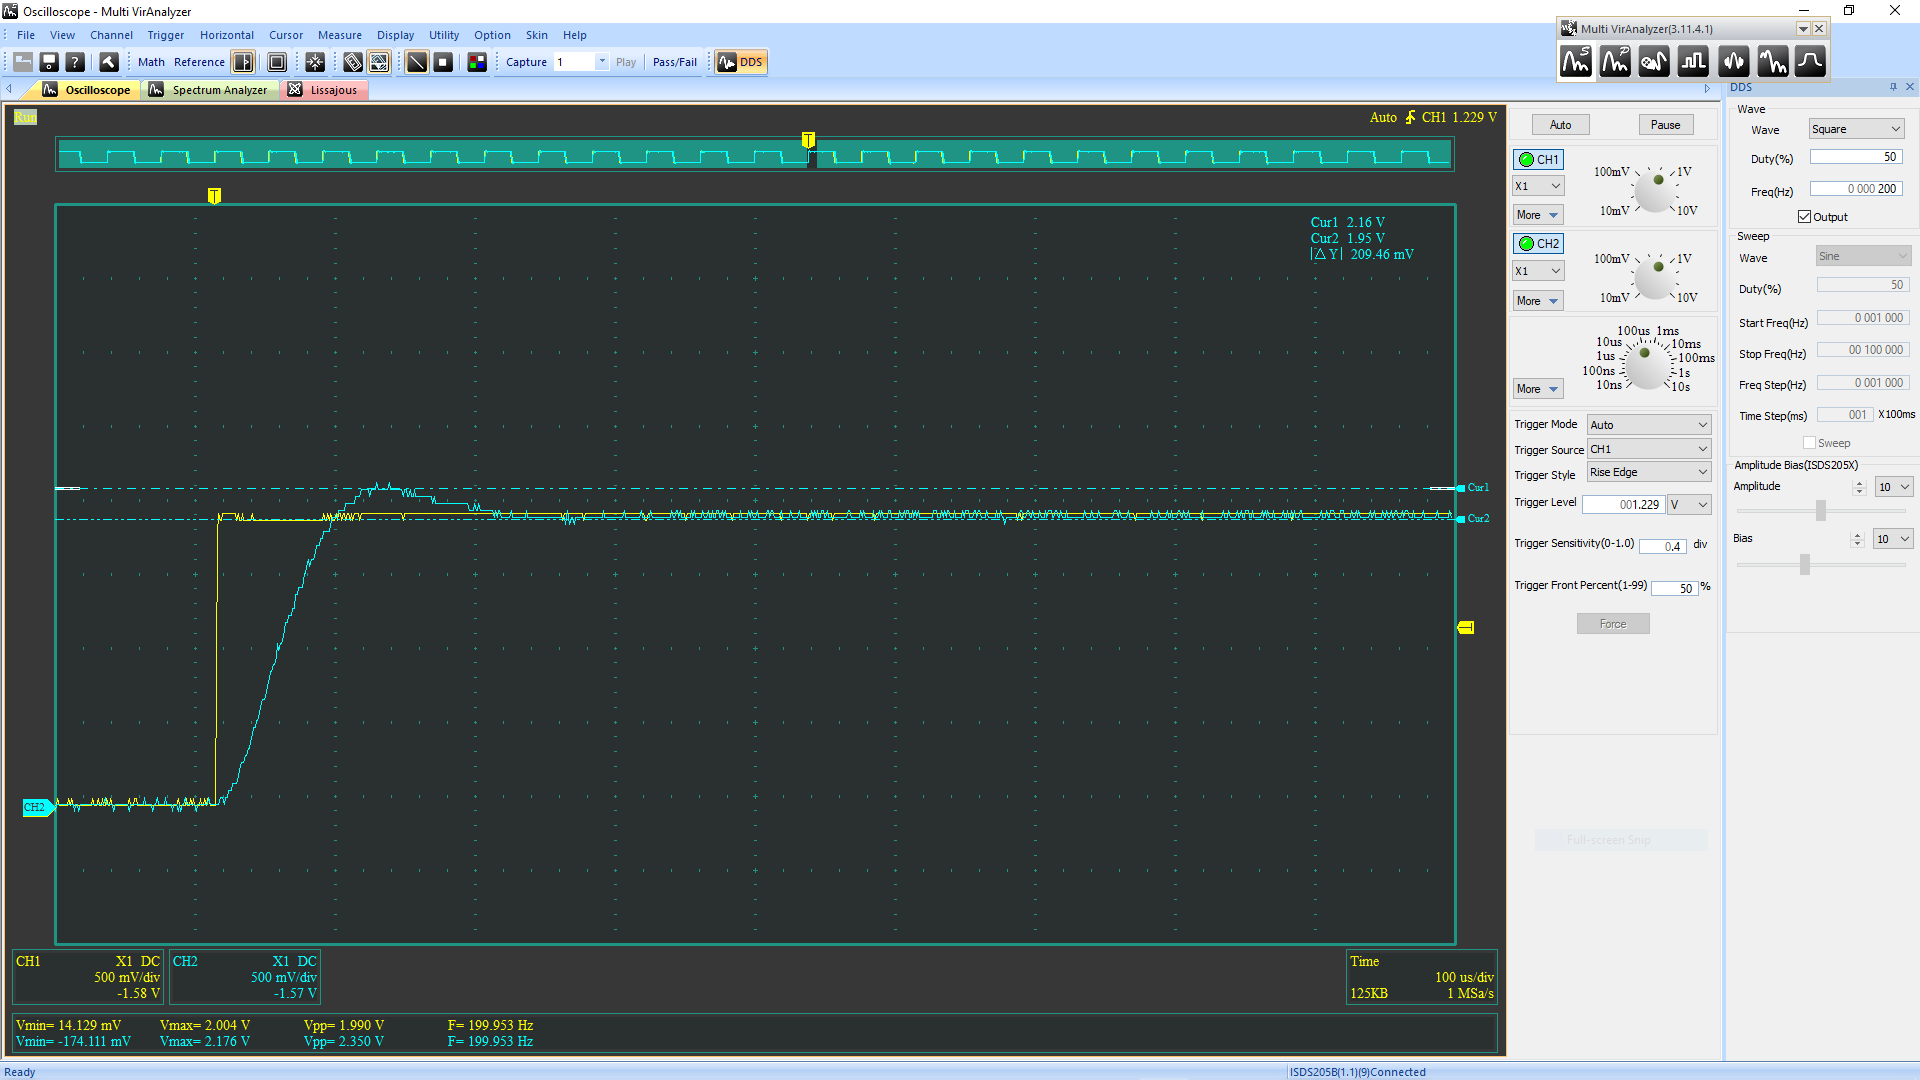
\includegraphics[width=\textwidth]{4.4 (0.6) 1.png}}
            {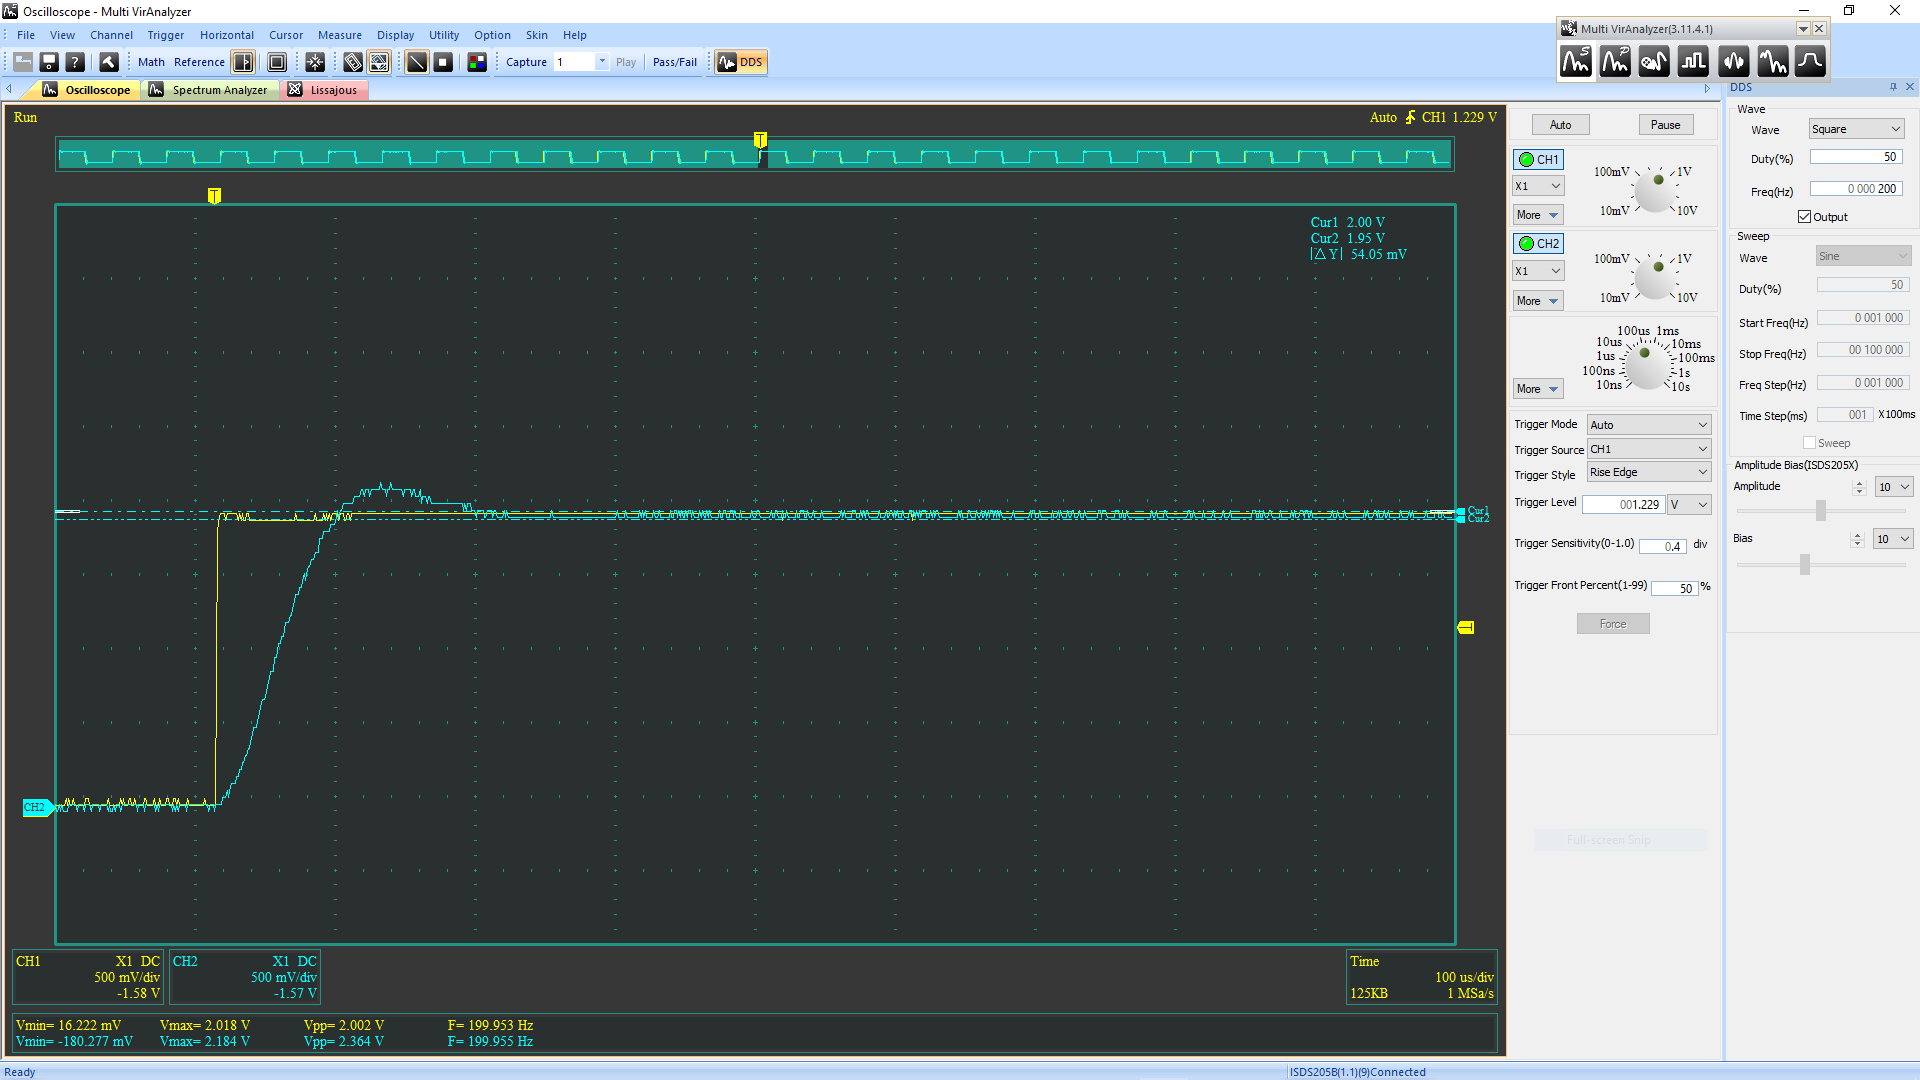
\includegraphics[width=\textwidth]{4.4 (0.6) 2.png}}
    \end{center}
    \begin{center}
        Figures 8 and 9: Step response when $ \zeta = 0.6 $, $ R = 3351.91 \Omega $
    \end{center}
    \newpage
    \begin{figure}[h]
        \centering
        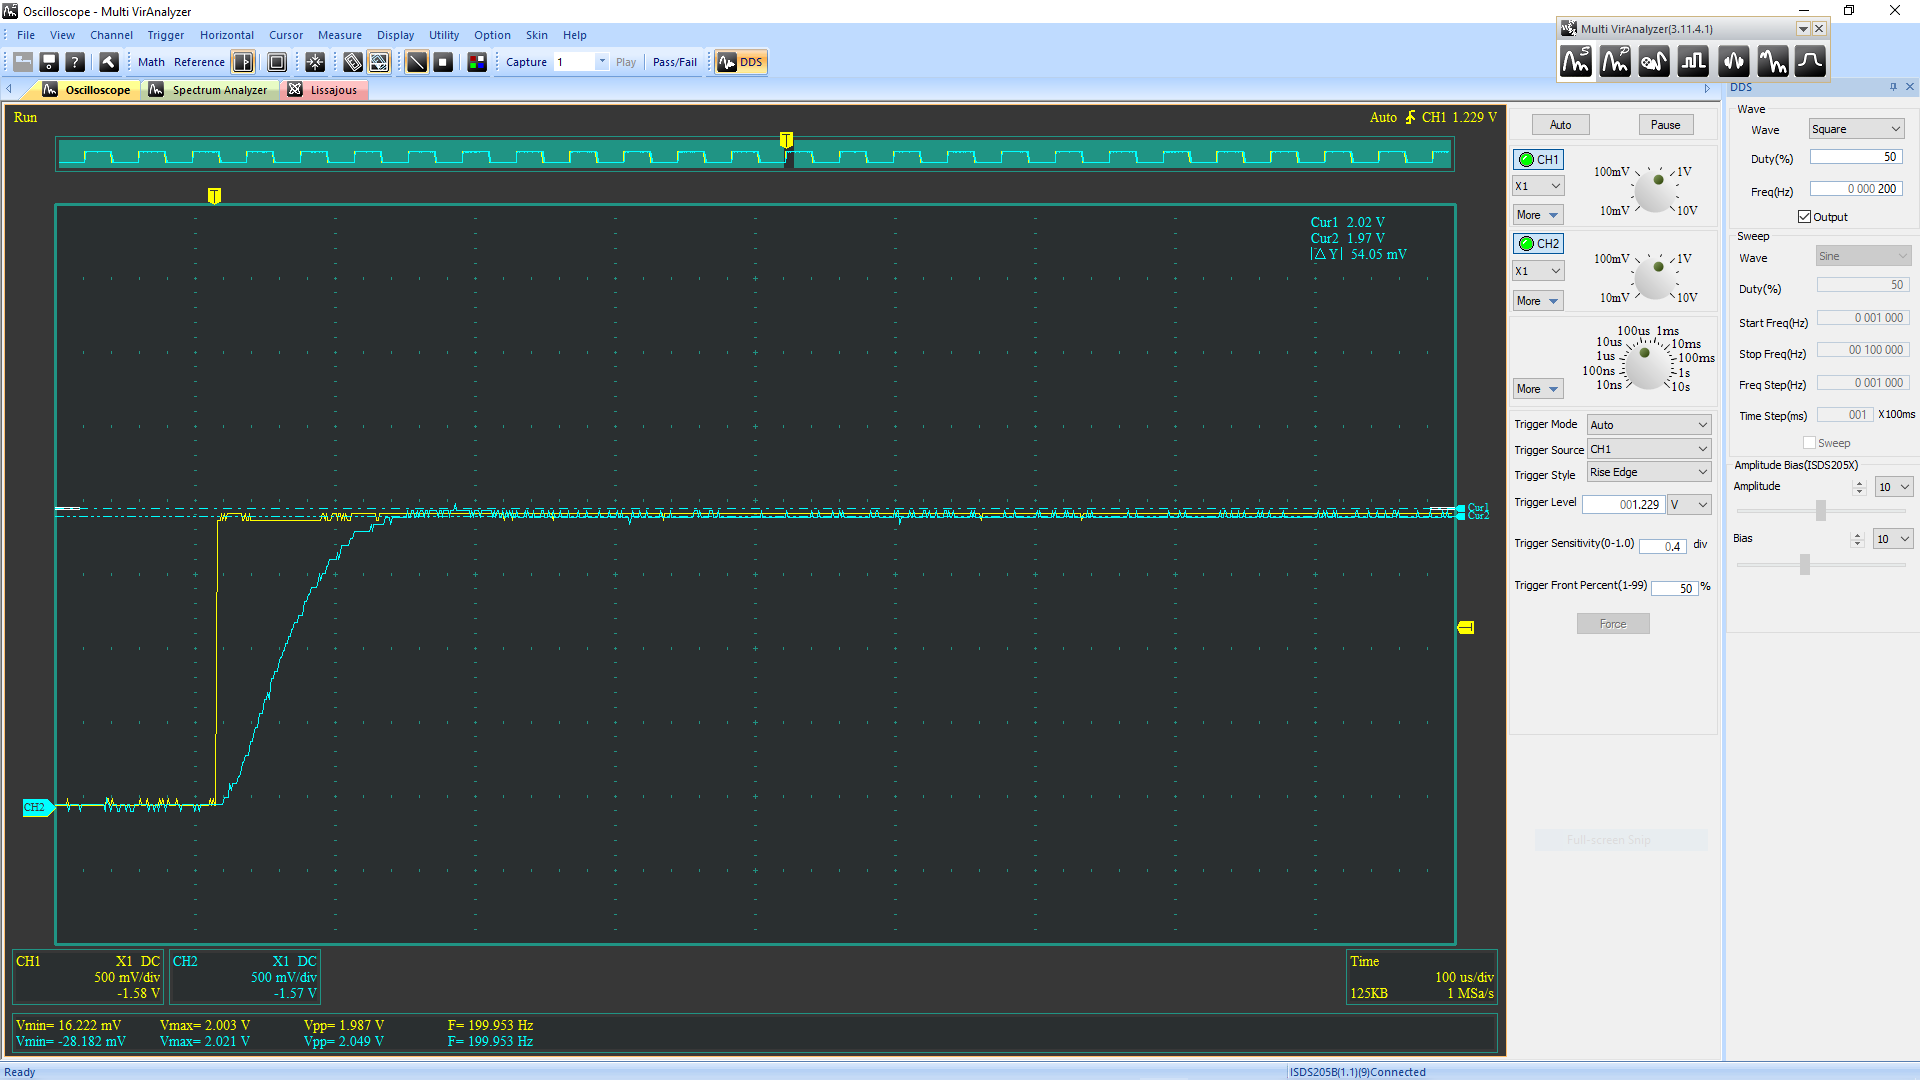
\includegraphics[width=0.9\textwidth]{4.4 (0.8).png}
    \end{figure}
    \begin{center}
        Figures 10: Step response when $ \zeta = 0.8 $, $ R = 4608.55 \Omega $
    \end{center}
    \begin{figure}[h]
        \centering
        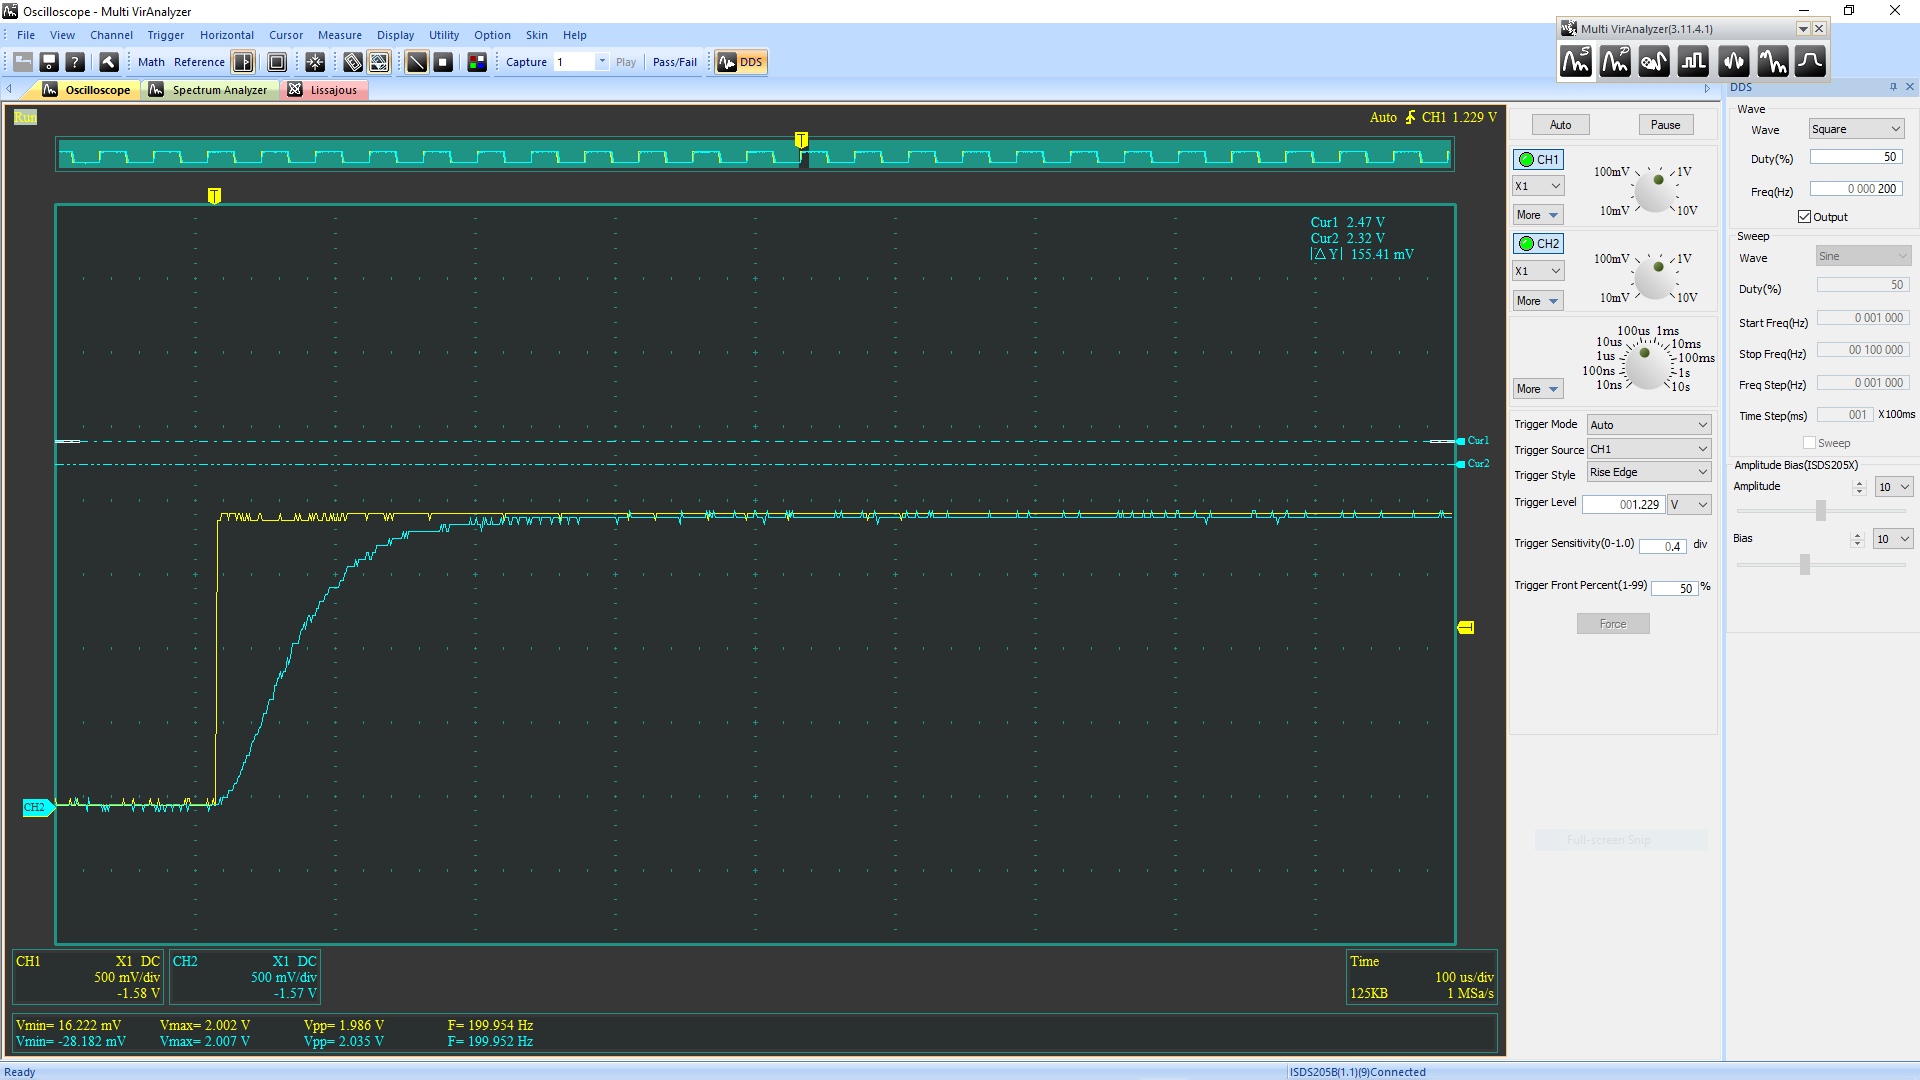
\includegraphics[width=0.9\textwidth]{4.4 (1.0).png}
    \end{figure}
    \begin{center}
        Figures 11: Step response when $ \zeta = 1.0 $, $ R = 5865.19 \Omega $
    \end{center}
    \newpage
    \begin{figure}[h]
        \centering
        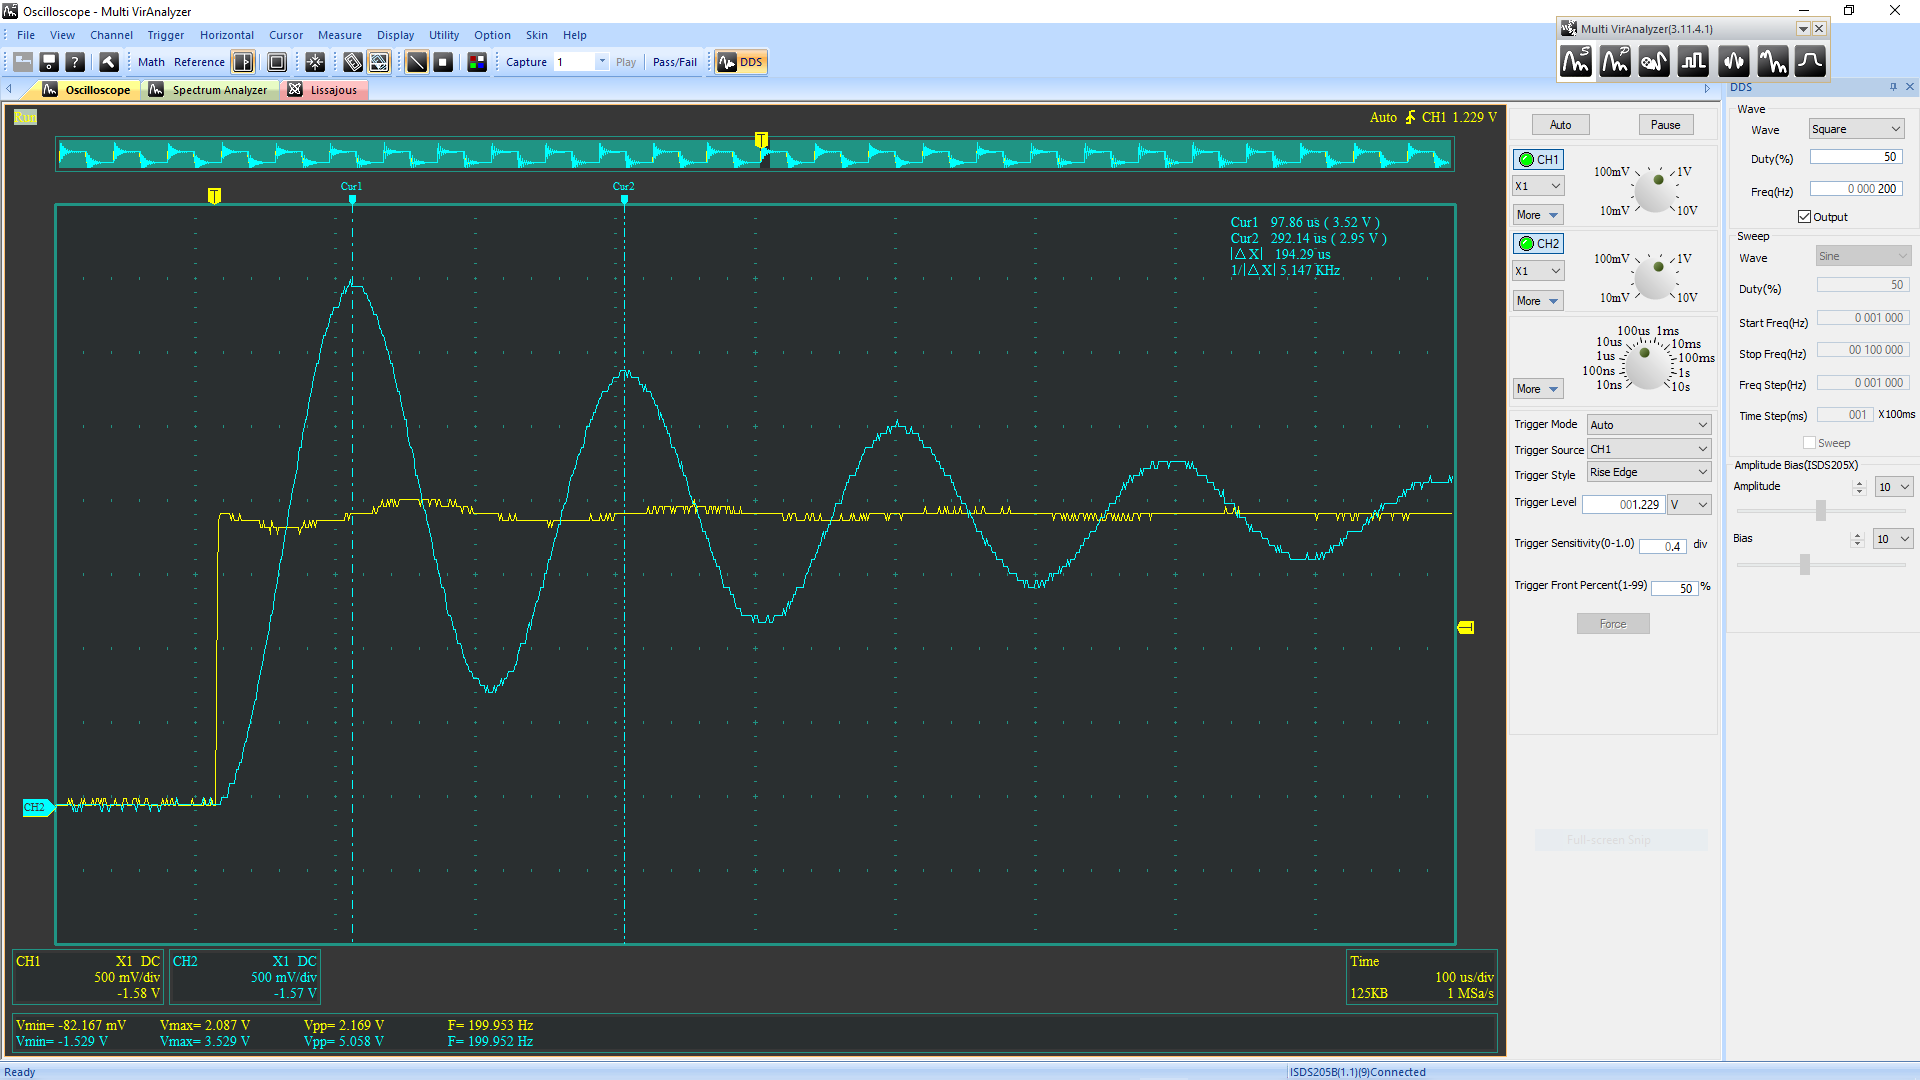
\includegraphics[width=0.9\textwidth]{4.5.png}
    \end{figure}
    \par Above is the waveform for the experiment 4.5. Here, the resistor is taken away completely and the only elements within the circuit are the inductor and the capacitor. The response can still be seen to be damped and this is due to the internal resistance of the components namely, the inductor and the function generator. To find the frequency in hertz from the waveform, we use the cursors. The period can be seen to be 194.29 $ \mu $s and taking the inverse, we get the frequency, 5.147 kHZ.
    \subparagraph*{Summary:}
    The function generator has an internal resistance and this resistance was found in the first experiment, 4.1. The circuit was setup as a voltage divider and at half of the peak to peak voltage with no resistance, the resistance provided by the resistor and the internal resistance of the generator must be the same. Using this principle, the value of the resistor at which this occurs, and thus the value of the function generator's resistance, was found to be 198 $ \Omega $. The resistance of the inductor was even simpler to determine and was done by simply using the multimeter across the inductor to determine its resistance. The internal resistance of the inductor was found to be 220 $ \Omega $. These two values needed to be subtracted from the theoretical values found for $ R $ in order to set the correct value for the variable resistor. In experiment 4.4, we changed the value of the damping coefficient by changing the value of $ R $ and with that, we were able to observe changes in the response of the circuit. In the end, the measured values were found to be close to the expected values from the formula. This is to be expected since there are factors such as the resistance of the wires and the noise induced by the low frequency square wave which all alter the measured values from the theoretical ones. Lastly, we found the natural frequency using the waveforms. This also was flawed due to the fact that there was resistance still in the circuit which likely made the results less accurate that the idealized cases. Nonetheless, the values determined and the waveforms generated were all close to the expected values with a degree of error. This suggests that the theoretical models used are sound approximations and that the experiments were conducted correctly.
\end{document}
